\chapter{测试与分析}
本章介绍测试的环境、使用的工具和测试的方法。测试结果表明,本安全删除方案能够保证在删除原始哈希信息后,
原始数据无法恢复;对仿真系统的带宽测试,对比固态盘的硬件性能,能够充分利用固态盘的I/O读写能力;系统I/O整体
时延比较小;系统负载属于正常水平,占用的计算资源和内存资源较为正常;加密后的数据冗余稳定在一个固定的范围内。
验证了本方案的可用性和可靠性。
\section{测试平台及环境说明}
测试环境使用的软硬件详细配置如\autoref{tab:test}所示。
\begin{table}[H]
    \centering
    \caption{测试环境配置}
    \label{tab:test}
    \begin{tabular}{|c|c|c|}
        \hline
        类别 & 型号 & 数量 \\ \hline
        CPU & Intel(R) Xeon(R) L5520  @ 2.27GHz & 单核16线程 \\ \hline
        内存 & 16GB & 1 \\ \hline
        密钥盘 & SV300S37A SATA3 120G & 1 \\ \hline
        数据盘 & SV300S37A SATA3 120G & 4 \\ \hline
        OS & Ubuntu 16.04.2 LTS & - \\ \hline
        内核 & Linux 4.4.0-75 & - \\ \hline
    \end{tabular}
\end{table}
\section{功能测试}
系统各项子功能测试结果如\autoref{tab:3}所示。
\begin{table}[H]
\centering
\caption{系统各项功能测试结果}\label{tab:3}
    \begin{tabular}{|*{4}{c|}}
\hline
        \textbf{操作} & \textbf{实验状态} & \textbf{结果} & \textbf{结论} \\ \hline
        \tabincell{c}{写入测试文件} & \tabincell{c}{密钥盘、数据盘均写入\\数据,加密数据与原始\\数据内容完全不同,\\且是不可读文本} & \tabincell{c}{加密功能正常,\\数据写入成功} & 写入子功能正常 \\ \hline
        \tabincell{c}{读取测试文件} & \tabincell{c}{密钥盘、数据盘有数据\\传输,解密还原的文件\\内容与原始文件\\一致} & \tabincell{c}{解密功能正常,\\数据读取成功} & 读取子功能正常 \\ \hline
        \tabincell{c}{安全删除\\密钥盘数据,\\尝试还原测试\\文件} & \tabincell{c}{系统还原获取的\\文件内容与原始文件\\不一致} & \tabincell{c}{元数据\\已经改变} & 安全删除子功能正常 \\ \hline
        \tabincell{c}{擦除其中\\两个数据盘上的\\数据,再次\\还原测试文件} & \tabincell{c}{系统解密过程\\出错,提示\\缺少文件数据} & \tabincell{c}{加密数据已\\被部分删除} & 安全删除子功能正常 \\ \hline
    \end{tabular}
\end{table}
\section{I/O带宽测试}
仿真方案处理I/O读取时,首先需要将盘阵中将一个数据单元对应的全部加密数据单元读取到内存中,同时在密钥盘中读取到这个数据块的原始哈希信息,才能进行解密操作得到原始数据单元。测试读取带宽就是衡量这个整体过程中数据处理的效率。读取带宽结果如\autoref{fig:21}所示。
\begin{figure}[H]
	\centering
	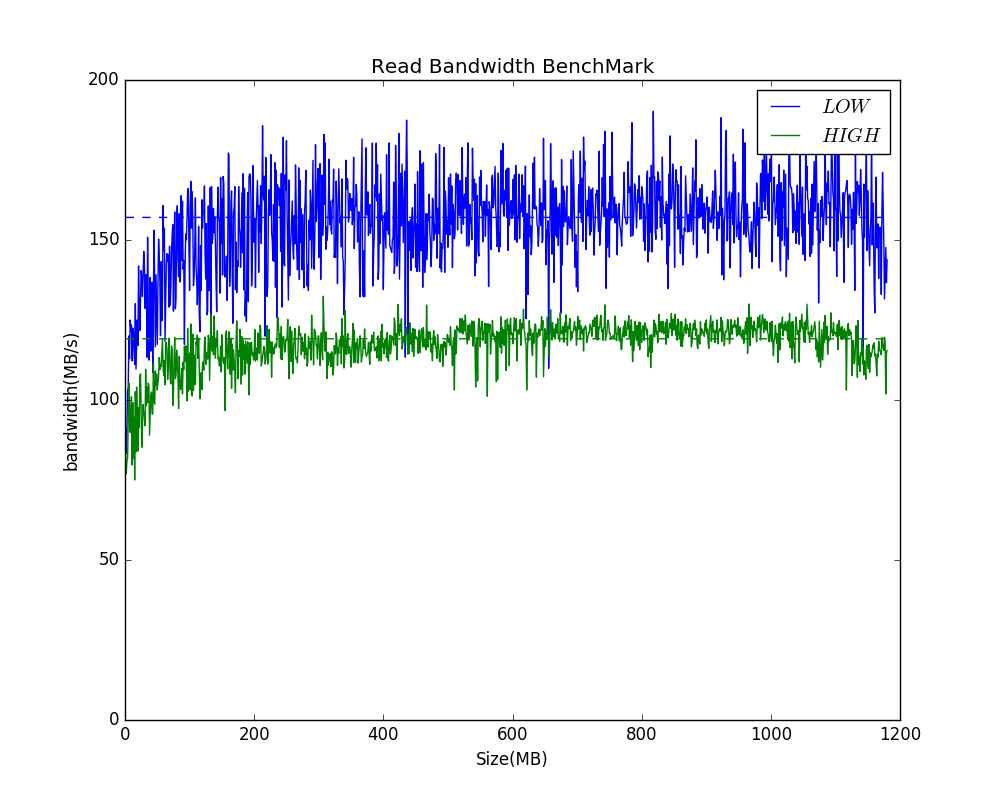
\includegraphics[width=1\textwidth,height=2.8in]{Pics/figure_bw_r.png}
	\caption{数据读取带宽}
	\label{fig:21}
\end{figure}
仿真系统处理数据写入时,首先将原始数据块按照预定义的数据大小分成一个个数据单元,根据系统的缓存参数和目标文件的大小来决定缓存的数据单元数量,并开始针对每个数据单元完成冗余加密操作,后端将缓存的加密数据单元按照次序写入阵列中存储,写入带宽衡量的是这整个过程中原始文件完成冗余加密存储的处理带宽。写入带宽测试结果如\autoref{fig:22}所示。
\begin{figure}[H]
	\centering
	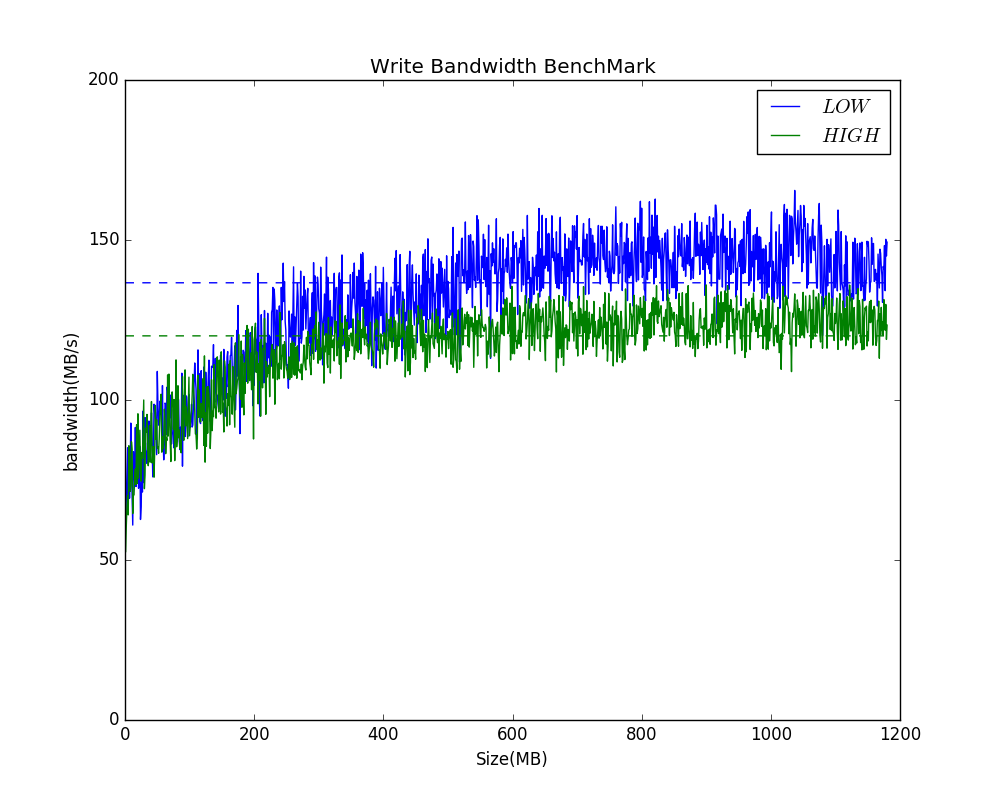
\includegraphics[width=1\textwidth,height=2.8in]{Pics/figure_bw_w.png}
	\caption{数据写入带宽}
	\label{fig:22}
\end{figure}


从读写带宽的测试结果可以看出,在一般加密级别下,数据读取带宽平均水平在158MB/s左右,而数据写入带宽大约为130MB/s。在高强度加密级别下,数据读写带宽整体都比一般加密级别要低一些,其中读取带宽大约是129MB/s,而写入带宽也是在120MB/s左右。


整体上,高强度加密级别的数据处理带宽比一般级别的要低,是因为数据单元在经过非对称加密的过程所耗费的时间要长,但是这种情况是在原始数据量大的情况下,此时加密模块的操作耗费时间成为仿真系统的主要瓶颈。在数据量较小时,二者的差别主要在数据预取和数据缓存的不同上,差别不是很大。


用于存储的SSD盘规格是读取速度为180MB/s,写入速度133MB/s。与原始盘的读写速度相比,仿真系统在写入状态下基本已经达到峰值,而读取状态的损失大约分别在12.2\%和33.3\%,考虑到日常使用对固态盘的损耗,方案的读取性能是可以接受的。


另外,仿真系统的读写带宽最终都稳定在平均水平附近,波动很小,可以得出,系统在处理数据带宽方面,具有一定的稳定性。
\section{I/O时延测试}
I/O延迟测试,在数据被读取时,是计量从发出请求,到缓存模块将第一个数据单元对应的加密数据单元全部取出,推送到解密模块处理的时间。读取时间延迟测试结果如\autoref{fig:23}所示。
\begin{figure}[H]
	\centering
	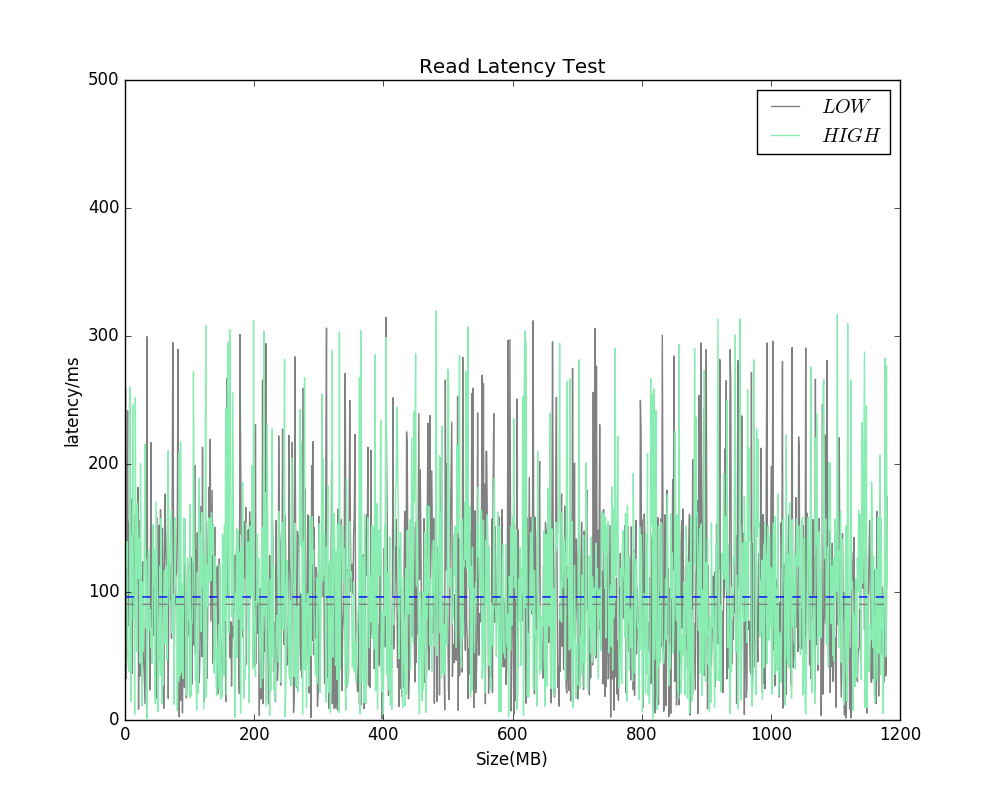
\includegraphics[width=1\textwidth,height=2.8in]{Pics/figure_lat_r.png}
	\caption{系统读取延迟}
	\label{fig:23}
\end{figure}
在写入数据时,是记录第一个数据单元推送到加密模块的时间。写入时间延迟测试结果如\autoref{fig:24}所示。
\begin{figure}[H]
	\centering
	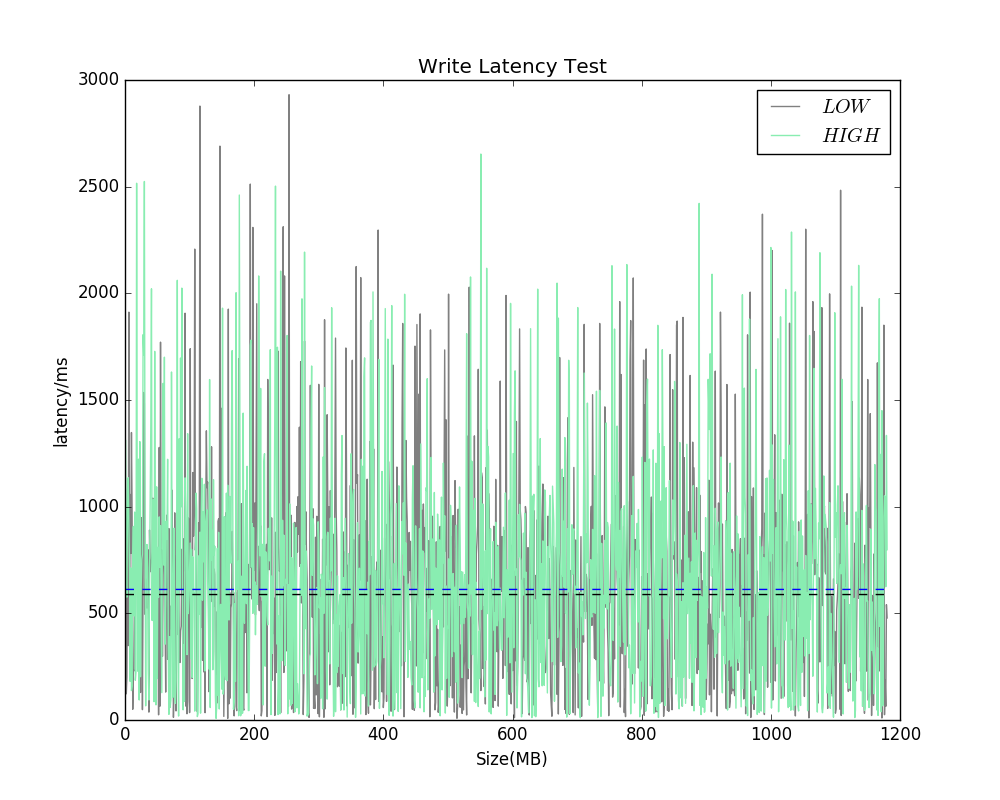
\includegraphics[width=1\textwidth,height=2.8in]{Pics/figure_lat_w.png}
	\caption{系统写入延迟}
	\label{fig:24}
\end{figure}
从时间延迟测试结果来看,仿真系统的读取延迟和写入延迟在不同加密级别下的差别很小,其中读取延迟大约为90ms左右,读取延迟最差不超过300ms。写入延迟均在600ms附近波动,最差情况不超过3000ms。两种测试情形下,系统时延波动都比较显著,然而大部分延迟数据都集中在平均水平,从这点来看,系统的时延也具有一定的稳定性。
\section{系统负载测试}
资源占用测试分为代表仿真系统需要的计算资源和内存资源,系统在对数据进行冗余加密时需要耗费更多的CPU时间片,在缓存读取数据和加密后数据时需要额外的内存空间,因此,从进程的CPU占用和内存占用就可以反映整体系统运行需要的环境。其中前端负载表示的主要是I/O请求、加密这些即时性的负载,后端表示的是数据存储、读取这些长时间的负载。系统不同安全级别下的CPU负载如\autoref{fig:25}和\autoref{fig:26}所示。
\begin{figure}[H]
	\centering
	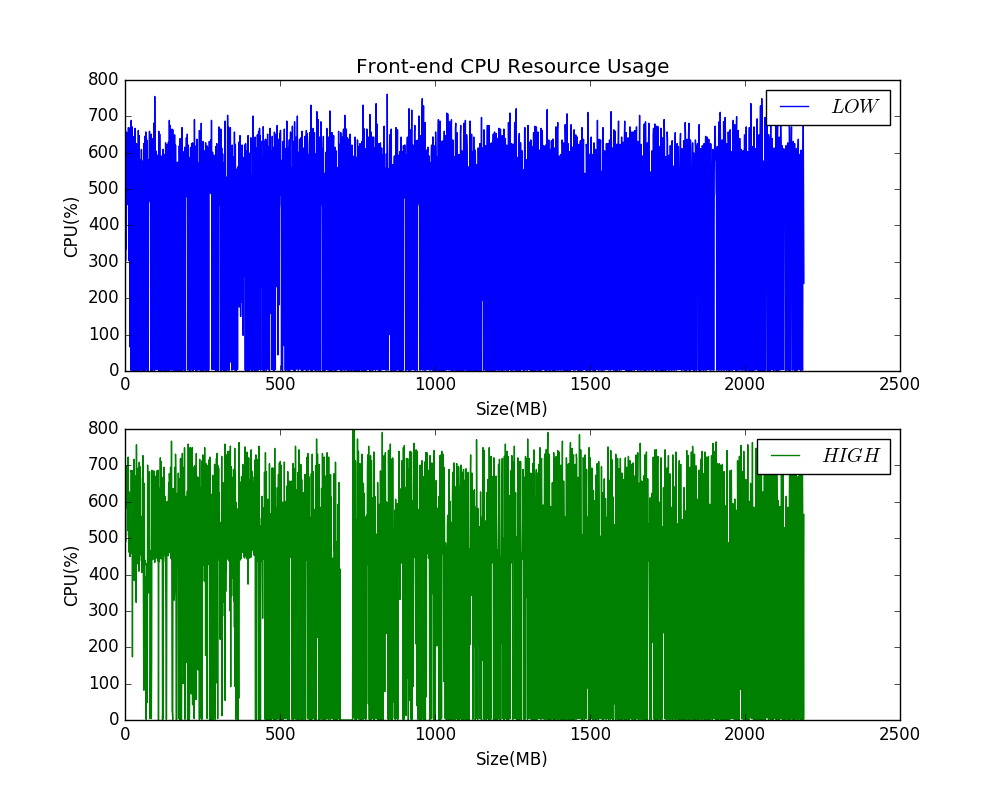
\includegraphics[width=1\textwidth,height=3.5in]{Pics/figure_cpu_client.png}
	\caption{系统前端CPU占用}
	\label{fig:25}
\end{figure}
\begin{figure}[H]
	\centering
	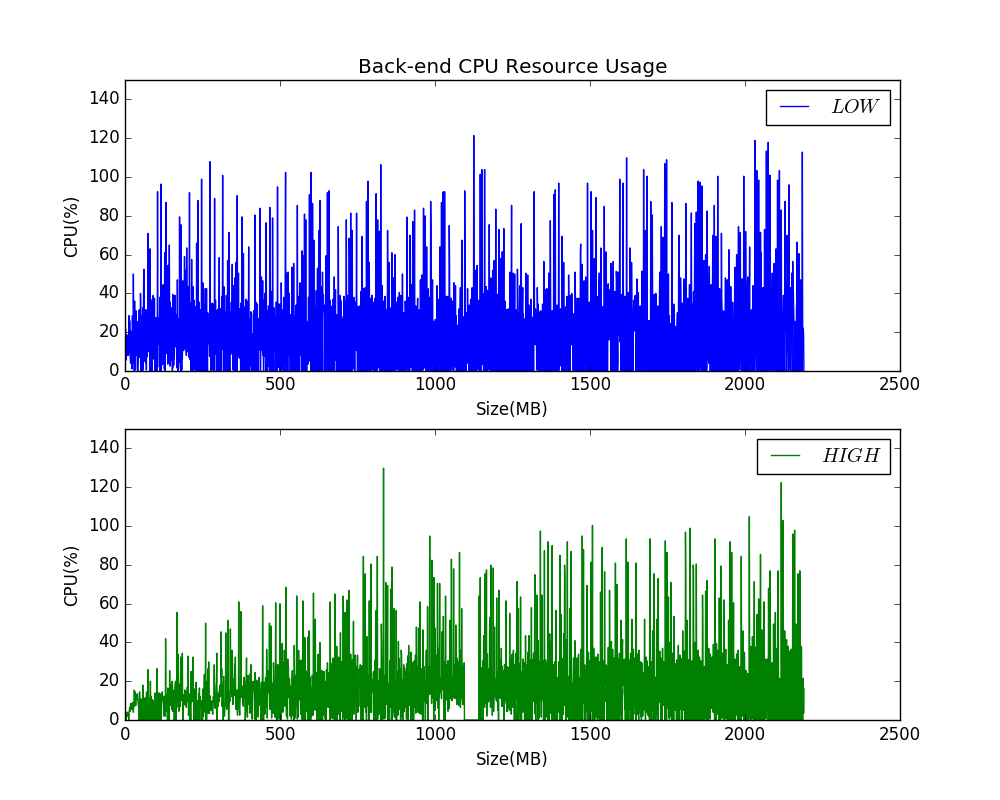
\includegraphics[width=1\textwidth,height=3.5in]{Pics/figure_cpu_server.png}
	\caption{系统后端CPU占用}
	\label{fig:26}
\end{figure}
前后端内存负载分别如\autoref{fig:27}和\autoref{fig:28}所示。
\begin{figure}[H]
	\centering
	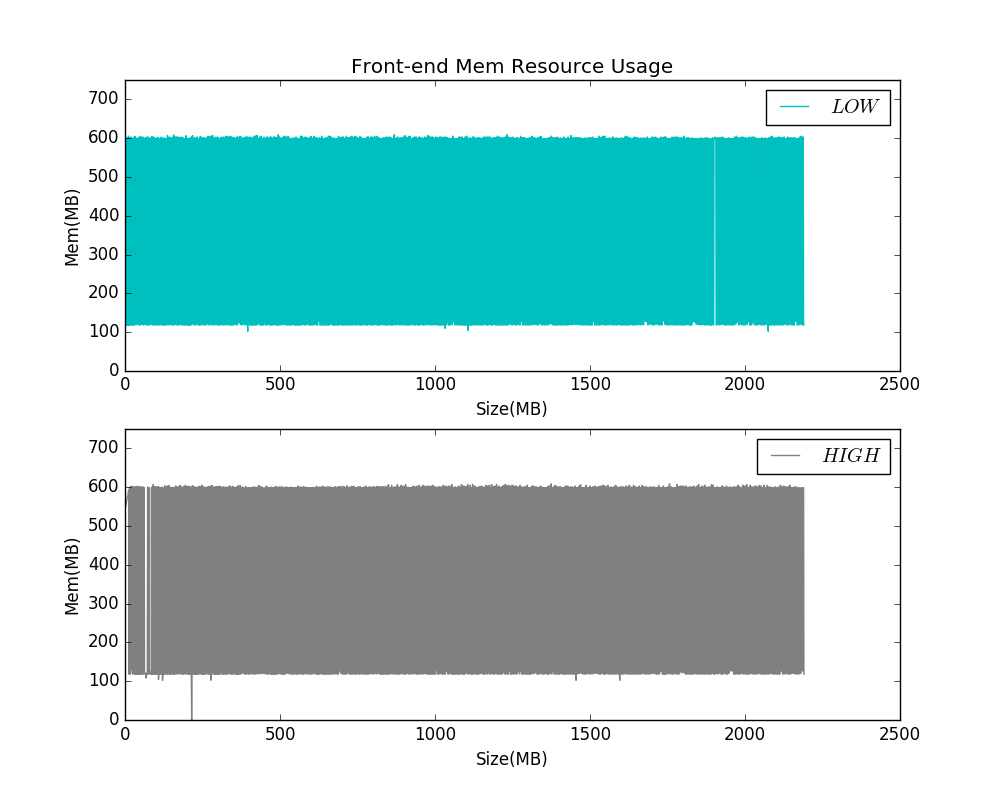
\includegraphics[width=1\textwidth,height=3.5in]{Pics/figure_mem_client.png}
	\caption{系统前端内存占用}
	\label{fig:27}
\end{figure}
\begin{figure}[H]
	\centering
	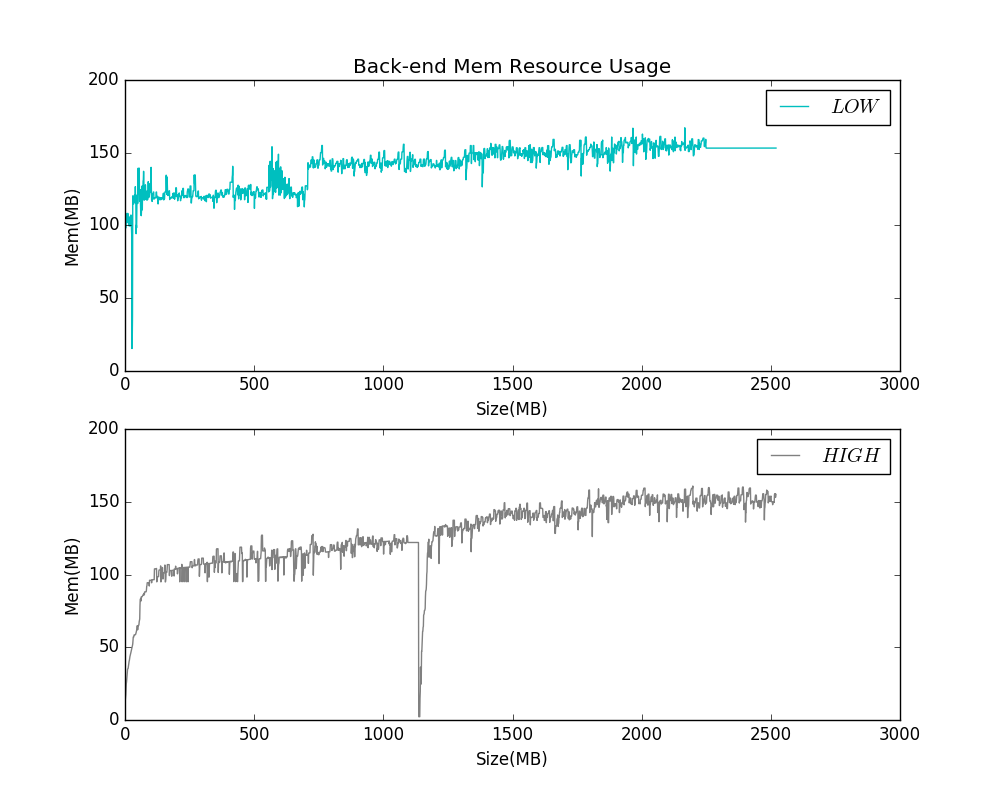
\includegraphics[width=1\textwidth,height=3.5in]{Pics/figure_mem_server.png}
	\caption{系统后端内存占用}
	\label{fig:28}
\end{figure}
从负载测试结果来看,由于前端处理的任务具有瞬时性,加密操作耗费计算资源,所以两种加密级别下的CPU占用都在0到700\%之间变化,内存负载也在100MB到600MB左右变动,可以推断,仿真系统空闲时,前端几乎不占用计算资源,内存占用也在100MB左右。前端总体负载差异较大。


后端处理的任务主要是数据的缓存,读写这些请求,具有长期性的特点,不同的I/O请求对其影响比较平稳,因此测试结果显示的数据趋势比较平缓,其中CPU负载保持在20\%-40\%,内存负载保持在100MB-150MB范围内。后端总体负载比较小且稳定。
\section{数据冗余率测试}
数据冗余表示加密后的数据总量相比原始数据大小的差值,与原始数据的比值,由于系统设计方案是一种冗余存储系统,一个原始数据单元经过处理后,会产生几份冗余的加密数据,因此通过这个比值来判断方案在数据存储层面的可用性,冗余率越低,加密数据占用的存储单元越少,方案的实用性就更好。不同大小的数据冗余率如\autoref{fig:29}所示。
\begin{figure}[H]
	\centering
	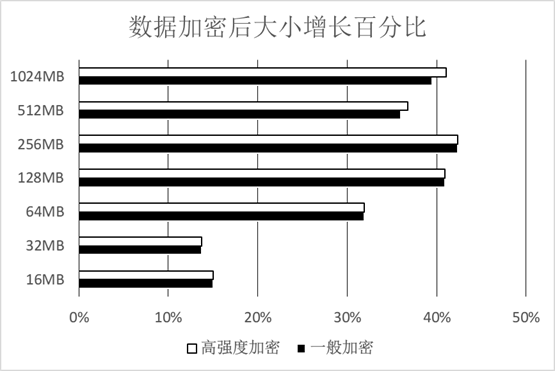
\includegraphics[width=1\textwidth]{Pics/data-ry.png}
	\caption{数据冗余率测试结果}
	\label{fig:29}
\end{figure}
两种强度加密系统,加密后的数据增长率在小文件(<16M)时,基本为0,而在中型文件(16M~64M)时大约为16\%~20\%,在大文件(>64M)时大约在38\%~41\%,不同大小的存储需求,系统的冗余率分为几个区间,在这些区间中变化。


结合上面的一些结论,可以发现,我们的安全删除方案不同安全级别的性能表现确实有差异;而且,整个系统基本可用。由于在物理上删除了元数据,在测试中原始数据无法恢复,系统提示错误。由此得到结论,如果彻底破坏了存储的元数据信息,数据是完全无法恢复的。同时,
在使用本系统中,由于元数据是原始数据块的哈希信息,相比冗余加密后的数据,其对应的元数据大小非常小,存储量不及前者的万分之一。因此,为了保证数据安全删除的效果,
删除元数据信息比删除冗余数据单元,对闪存物理单元的磨损要小很多,达到了本方案提到的减少闪存磨损的优势。


功能测试部分确保了方案的写入、读取、加密、删除功能是可以正常工作并且产生预期效果的,也就是证明了我们方案的有效性。


系统测试分别从带宽、时延、负载、冗余量这四个维度,详细测试了系统的相关性能,根据测试结果的表现并加以分析,初步证明了方案的可行性、可靠性。

\section{本章小结}
本章对全闪存盘阵数据安全删除的仿真系统进行了功能测试和性能测试,测试平台采用的是仿真实验的实现平台,
功能测试部分主要测试了仿真系统的写入、读取、安全删除这些子功能,验证了系统在安全删除关键信息后,数据
无法恢复的方案要求。性能测试部分通过对系统处理带宽、I/O时延、系统负载和冗余率的测试,验证了系统的可行性、可靠性。
同时,安全删除元数据达到数据安全删除的目的,显著降低了闪存物理磨损单元,也就延长了固态盘的使用寿命。
